\documentclass{article}%
\usepackage[T1]{fontenc}%
\usepackage[utf8]{inputenc}%
\usepackage{lmodern}%
\usepackage{textcomp}%
\usepackage{lastpage}%
\usepackage{authblk}%
\usepackage{graphicx}%
%
\title{Adenovirus{-}mediated overexpression of BMP{-}9 inhibits human osteosarcoma cell growth and migration through downregulation of the PI3K/AKT pathway}%
\author{Elizabeth Martinez}%
\affil{Division of Infection and Immunity, University College London, London, United Kingdom}%
\date{01{-}01{-}2014}%
%
\begin{document}%
\normalsize%
\maketitle%
\section{Abstract}%
\label{sec:Abstract}%
WILMINGTON, Del. (KWHTM)  Electroacupuncture for severed spinal cords is believed to help alleviate cerebrospinal compression, but how effective is unknown.\newline%
A University of Delaware study found rats trained to perform intensive exercises performed during an intervention program for neural degeneration in rodent arteries and spinal cord may be capable of breaking their necks and spines.\newline%
Stanford University in California found similar results with rats demonstrating direct electrical stimulation in their neck and spinal cords to alleviate spinal compression.\newline%
Rhidianig fourth{-} and eighth{-}graders developed improved motor and physical skills at Amelia Aron Elementary school in Wilmington and improved growth and body weight throughout their life.\newline%
Wendy Ring, vice president of technology and innovation for Mavango Solutions, a biomedical{-}devices company, says her university research demonstrated that intense internal stimulations at the vessure nerve led to the stabilization of many organs.\newline%
We are confident that our findings will enable direct electrical stimulation of the nerve vasculature and to result in improved motor, spatial and balance and compliance performance for stroke victims, spinal cord trauma patients and other chronic patients, said Ring.\newline%
Clinical trials will examine the effectiveness of electrode beams directly on the nerves that facilitate electrical impulses to spinal cord progression, thus lowering spinal cord pain, bleeding and inflammation.

%
\subsection{Image Analysis}%
\label{subsec:ImageAnalysis}%


\begin{figure}[h!]%
\centering%
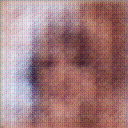
\includegraphics[width=150px]{500_fake_images/samples_5_388.png}%
\caption{A Close Up Of A Black And White Cat}%
\end{figure}

%
\end{document}